% !TeX spellcheck = de_CH_frami

\section{Graphen\label{sec:sgwt:graphs}}
\rhead{Graphen}

Graphen stellen eine weit verbreitete M\"oglichkeit dar, wie wir unsere Daten 
miteinander sinnvoll in Verbindung bringen. Ein Graph $G$ setzt sich aus einer 
Menge von Knoten $V$ und einer Menge von Kanten $E$ zusammen.
\begin{equation*}
G = \{V, E\}
\end{equation*}
Die jeweiligen Kanten $E$ verbinden jeweils genau zwei Knoten der zum Graph 
geh\"orenden Knotenmenge $V$ miteinander.
\begin{equation}
E \subset \{\{v_1, v_2\} | v_i \in V, v_1 \neq v_2 \}
\label{eq:sgwt:graph:def}
\end{equation}

\subsection{Ungerichtete Graphen}

Aus der von uns gew\"ahlten Definition eines Graphen 
in~\cref{eq:sgwt:graph:def} ist ersichtlich, dass es sich dabei um einen 
ungerichteten Graphen handelt, da die Reihenfolge von $v_1$ und $v_2$ keine 
Rolle spielt. \Cref{fig:sgwt:graph:simple} zeigt solch einen ungerichteten 
einfachen Graphen mit f\"unf Knoten und vier Kanten, die diese verbinden.

\begin{figure}
    \centering
    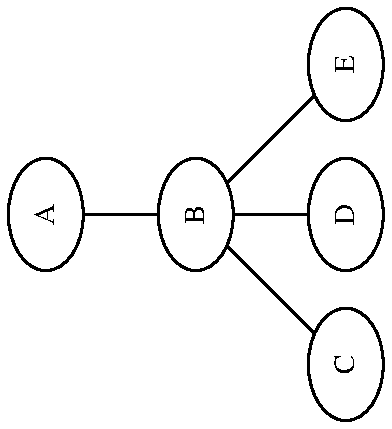
\includegraphics[
    angle=-90,
    origin=c,
    scale=0.7
    ]{papers/sgwt/images/simplegraph.pdf}
    \vspace{0pt}
    \caption{Beispiel eines einfachen ungerichteten Graphen mit f\"unf Knoten 
        und vier Kanten. Der zentrale Knoten $B$ hat hier den h\"ochsten Grad, 
        da er die gr\"osste Anzahl Verbindungen zu anderen Knoten hat.
        \label{fig:sgwt:graph:simple}}
\end{figure}

Zu den grundlegenden Eigenschaften eines Graphen geh\"ort der Grad eines jeden 
Knotens. Dieser entspricht der Anzahl Kanten, von denen dieser Knoten ein 
Teil ist.
\begin{equation*}
    d(v) = | \{e \in E | v \in e \} |
\end{equation*}
Bei unserem Beispielgraphen aus~\cref{fig:sgwt:graph:simple} 
erhalten wir somit folgende Grade f\"ur die jeweiligen Knoten: $d(A) = 1, d(B) 
= 4, d(C) = 1, d(D) = 1, d(E) = 1$.

\subsection{Gewichtete Graphen}

Den einzelnen Kanten ein Gewicht zu geben, ist eine M\"oglichkeit, 
zus\"atzliche Informationen in einem Graphen zu hinterlegen. Jeder ungewichtete 
Graph kann auch als ein gewichteter Graph, dessen Kanten einfach jeweils ein 
Gewicht von $1$ haben, gesehen werden.

Bei gewichteten Graphen wird auch der Grad eines Knotens zu einem gewichteten 
Grad. Das heisst, dass nun nicht mehr einfach die Anzahl Kanten von Bedeutung 
ist, sondern auch das jeweilige Gewicht der Kante. Der gewichtete Grad eines 
Graphen ist also die Summe aller Kantengewichte, die den jeweiligen Knoten 
beinhalten. 
\begin{equation*}
    d_w(v) = \sum_{i = 1}^{|E|}w(e_i), \qquad v \in e_i
\end{equation*}
Nehmen wir wieder den Beispielgraphen aus~\cref{fig:sgwt:graph:simple} und 
versehen die einzelnen Kanten mit Gewichten. Damit erhalten wir dann den 
Graphen in~\cref{fig:sgwt:graph:simpleweight}. Die Gewichte sind dabei 
willk\"urlich gew\"ahlt worden, sie k\"onnen aber auch einen realen Hintergrund 
haben, zum Beispiel die inverse Luftliniendistanz zweier Ortschaften. Der Grade 
f\"ur die jeweiligen Knoten sind somit: $d_w(A) = 1, d_w(B) = 3.4, d_w(C) = 
1.2, d_w(D) = 0.4, d_w(E) = 0.8$.

\begin{figure}
    \centering
    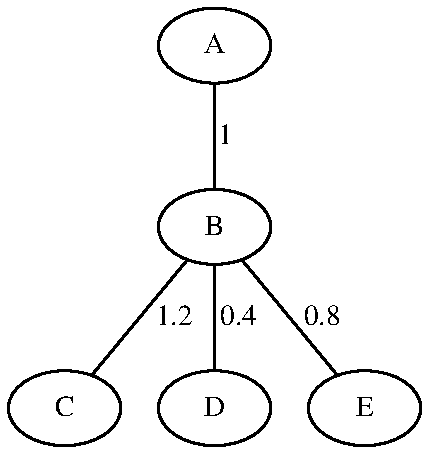
\includegraphics[
    scale=0.7
    ]{papers/sgwt/images/weightedsimplegraph.pdf}
    \vspace{0pt}
    \caption{Beispiel eines einfachen gewichteten Graphen mit f\"unf Knoten 
        und vier Kanten. Der zentrale Knoten $B$ hat hier, wie schon 
        in~\cref{fig:sgwt:graph:simple}, den h\"ochsten Grad.
        \label{fig:sgwt:graph:simpleweight}}
\end{figure}

\subsection{Funktionen auf Graphen}

Was uns eigentlich aber wirklich interessiert, ist das Abbilden von Funktionen 
auf Graphen. Das heisst, wir weisen den jeweiligen Knoten einen Wert unserer 
Funktion zu.
\begin{equation*}
f(v) = \dots, \qquad v \in V
\end{equation*}

Nehmen wir eine Funktion die an den f\"unf Punkten $x_1$ bis $x_5$ auf der 
$x$-Achse abgetastet wurde. Diese Funktion k\"onnen wir einfach auf einen 
Graphen abbilden, indem wir die einzelnen Punkte auf der $x$-Achse als Knoten 
eines Graphen sehen und diese mit einfachen Kanten verbinden. Wir k\"onnen 
diese Kanten auch gewichten, zum Beispiel in dem wir jeweils die Differenz 
zwischen zwei Punkten nehmen. Schlussendlich haben wir dann etwas in der Form 
des Graphen in~\cref{fig:sgwt:graph:fungraph}. Dabei sind die Funktionswerte 
nicht mehr direkt ersichtlich, sondern wurden mit Farben kodiert.

\begin{figure}
    \centering
    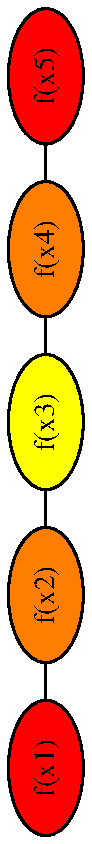
\includegraphics[
    angle=-90,
    origin=c,
    scale=0.7
    ]{papers/sgwt/images/fungraph.pdf}
    \vspace{-120pt}
    \caption{Beispiel von Funktionen die auf einem Graphen liegen. Die 
    Funktionswerte sind hier farblich dargestellt. Die Variable 
    $x_1$ bis $x_5$ sind dann statt Punkte auf einem Zahlenstrahl, einzelne 
    Knoten eines Graphen.
        \label{fig:sgwt:graph:fungraph}}
\end{figure}

\subsection{Linien-, Ring- und Kugelgraphen}

In den weiteren Abschnitten wird immer wieder von Linien-, Ring- und 
Kugelgraphen gesprochen. Damit gemeint ist jeweils eine Approximation einer 
Linie, eines Ringes oder einer Kugel mittels eines ungewichteten Graphen. 
\Cref{fig:sgwt:graph:ring,fig:sgwt:graph:line,fig:sgwt:graph:sphere} 
illustrieren die jeweiligen Graphen anhand eines Beispieles.

\begin{figure}
    \centering
    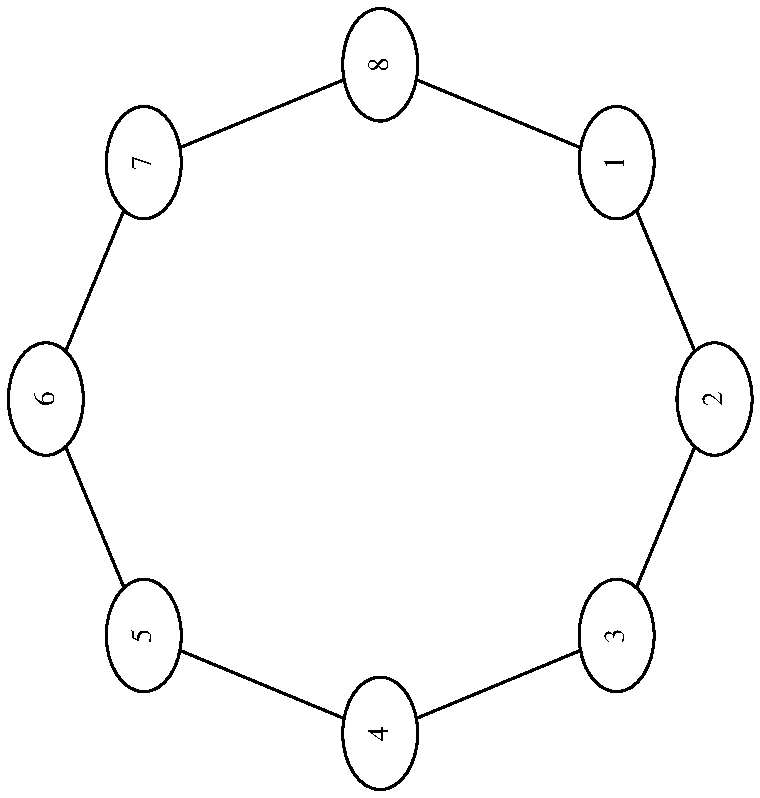
\includegraphics[
    angle=-90,
    origin=c,
    scale=0.6
    ]{papers/sgwt/images/ring-graph.pdf}
    \caption{Graph Approximation eines Ringes oder auch eines periodisch 
    fortgesetzten Signales.
    \label{fig:sgwt:graph:ring}}
\end{figure}

\begin{figure}
    \centering
    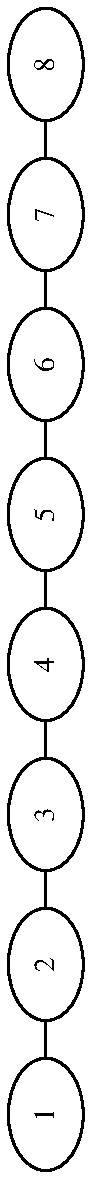
\includegraphics[
    angle=-90,
    origin=c,
    scale=0.6
    ]{papers/sgwt/images/line-graph.pdf}
    \vspace{-160pt}
    \caption{Graph Approximation einer einfachen Linie. Speziell sind dabei die 
    Endknoten, die jeweils nur den Grad $1$, statt $2$ wie alle anderen Knoten, 
    haben. 
    \label{fig:sgwt:graph:line}}
\end{figure}

\begin{figure}
    \centering
    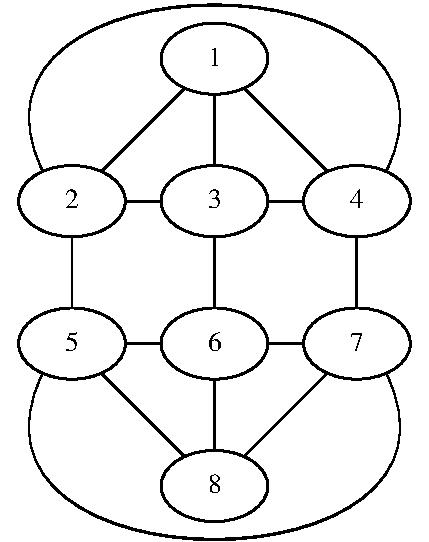
\includegraphics[
    scale=0.6
    ]{papers/sgwt/images/sphere-graph.pdf}
    \caption{Graph Approximation einer Kugel. Zu beachten gilt, dass der Grad 
    der beiden Polknoten jeweils stark vom Grad aller andere Knoten abweichen 
    kann.
    \label{fig:sgwt:graph:sphere}}
\end{figure}
